%%%%%%%%%%%%%%%%%%%%%%%%%%%%%%%%%%%%%%%%%%%%%%%%%%%%%%%%%%%%%%%%%%
%%%%%%%% CPSC 63 AI FINAL  REPORT %%%%%%%%%%%%%%%%%%%%%%%%
%%%%%%%% This template is modified from ICML 2014 %%%%%%%%%%%%%%%%
%%%%%%%%%%%%%%%%%%%%%%%%%%%%%%%%%%%%%%%%%%%%%%%%%%%%%%%%%%%%%%%%%%

\documentclass{article}

%include any external packages here.  This is similar to loading a
%library in python or C++

% use Times
\usepackage{times}
% For figures
\usepackage{graphicx}
\usepackage{subfigure}
% \usepackage{subcaption}

% For citations
\usepackage{natbib}

% For algorithms and pseudocode
\usepackage{algorithm}
\usepackage{algorithmic}

%Adds hyperlinks to your citations automatically
\usepackage{hyperref}

% Packages hyperref and algorithmic misbehave sometimes.  We can fix
% this with the following command.
\newcommand{\theHalgorithm}{\arabic{algorithm}}

\usepackage[accepted]{icml2014}
\usepackage{amsmath}


% If your title is long (below), use this command to also provide
% short version.  This will go on the top of every page
\icmltitlerunning{Final Report}

\begin{document}

\twocolumn[ %use two column if you need a text to span across the whole page
\icmltitle{ CS63 Spring 2025 \\ % \\ force a new line
Fine-Tuning YOLOv3 for Object Detection in Google reCAPTCHA v2 Image Challenges }

\icmlauthor{Victor Sumano Arango}{vsumano1@swarthmore.edu}
\icmlauthor{Nicholas D'Andrea}{ndandre1@swarthmore.edu}

\vskip 0.3in
]

\begin{abstract}
We developed a system that combined a custom YOLOv3-based real-time object detection model with a genetic algorithm (GA) for hyperparameter optimization to identify objects in Google’s reCAPTCHA v2 challenges, such as crosswalks, chimneys, and stairs. We pretrained our YOLOv3 model on a subset of annotated images from the COCO80 dataset and fine-tuned it using labeled images from reCAPTCHA v2. During training, we collected metrics including training loss, class accuracy, object accuracy, no-object accuracy, and mean average precision (mAP). To evaluate performance, we also trained and assessed the Ultralytics YOLOv5s model using pre-trained COCO80 weights in the same data set. Our custom YOLOv3 system consistently produced accurate bounding-box predictions for the target object categories, reaching 90\% class accuracy; however, it achieved MAP: 0.2912@0.3. Despite the low mAP, our results suggested that the GA-optimized YOLOv3 model offered more precise classification performance than YOLOv5s under similar training configurations.
\end{abstract}

\section{Introduction}
\label{introduction}
Before recent hardware and software breakthroughs, object detection relied primarily on traditional feature-based algorithms. One of the earliest methods, sliding windows, involved scanning an image with a fixed-size window that moved across every possible position, checking each window to determine if an object was present. Four years later, in 2008, Deformable Part Models (DPM) advanced the field further by breaking objects into parts, each represented by a bounding box, allowing for a more flexible and robust detection process. \cite{felzenszwalb2008discriminatively} Following the AI boom and the subsequent surge in interest in Convolutional Neural Networks, R-CNNs became the object detection standard. \cite{girshick2014rich} Then in 2016, YOLO (You Only Look Once) revolutionized object detection due to its speed and efficiency compared to any other model that came before it. \cite{redmon2018yolov3}

YOLO's introduction marked a significant shift in object detection methodology. Unlike earlier models that relied on region proposals followed by classification, YOLO reframed object detection as a single regression problem, predicting bounding boxes and class probabilities directly from full images in a single network pass. This end-to-end architecture enabled real-time performance without sacrificing much accuracy, establishing a new benchmark for speed and simplicity. Since then, convolutional neural networks (CNNs) have become the standard backbone architecture in nearly all modern object detection frameworks.

Today, object detection algorithms are fundamental in a wide range of applications, including real-time threat detection, autonomous navigation, facial recognition, and medical imaging. 

In this study, we investigate the use of a custom YOLOv3-based model to identify specific object categories, particularly crosswalks, chimneys, and stairs, commonly found in Google’s reCAPTCHA v2 image challenges. Google reCAPTCHA v2 is a widely deployed CAPTCHA service that differentiates between human users and automated bots by combining risk analysis with user interaction. When user behavior appears suspicious, the system presents an image-based challenge, often requiring users to select images containing particular objects.

Our approach involves training a customized YOLOv3 model using a subset of the COCO80 dataset, followed by fine-tuning on a dataset derived from reCAPTCHA v2 challenges. The training process draws on implementation details from both the original YOLOv3 paper and community-developed tutorials, with the goal of achieving robust performance on this object detection task.
\section{Methods}
\label{methods}
\subsection{YOLOv3}
\subsubsection{COCO80 and Google reCaptcha v2 datasets}
We utilized images from the COCO80 dataset and fine-tuned our models using approximately 500 annotated images from a Google reCaptcha v2 dataset. Due to time constraints, we extracted a subset of the 200k annotated images to speed up pre-training extracting a maximum of 2,000 images per class. To first pretrain our model, we preprocessed our data by converting the json files into .txt files for each image in our dataset. We then split the images to training and validating folders. 

For the Google reCaptcha v2 dataset, we divided the 500 annotated images into training, validation, and test sets with a 60/20/10 split.

\subsubsection{Data Augmentation}
We applied data augmentation using the Albumentations Python library during pretraining on the COCO80 dataset, but more importantly, we performed extensive augmentations on our Google reCAPTCHA v2 training data. Since our data set was highly imbalanced and limited in size, these increases were crucial to generate additional training samples from available images and to improve the model's ability to generalize.

During training, we resized and padded images, applied random cropping, and adjusted color properties such as brightness, contrast, and saturation. We also used Geometric transformations like rotation, scaling, and flipping to increase variation. For testing, we focused on resizing, padding, and normalization to ensure consistency without introducing randomness.

\subsubsection{Darknet-53 Backbone}
The implementation details and insights for Darknet-53 were adapted from the tutorial provided by Aladdin Persson. \cite{persson2021darknet53} This resource was instrumental in guiding the integration of Darknet-53 into our YOLO model. Our Darknet-53 architecture consists of 53 convolutional layers, each followed by a Batch Normalization (BN) layer to stabilize training and accelerate convergence.

To further improve learning efficiency, we apply the Leaky ReLU activation function after each convolutional layer. Unlike standard ReLU, Leaky ReLU maintains a small, nonzero gradient for inactive units, which helps mitigate the "dying ReLU" problem, a common issue where neurons become inactive and output zero for all inputs, effectively ceasing to learn. By allowing a small gradient when the unit is not active, Leaky ReLU helps keep these neurons involved in the learning process. Furthermore, we incorporate dropout with a probability of 0.2 to reduce the risk of overfitting by randomly deactivating neurons during training.

Darknet-53 also addresses the vanishing gradient problem through the use of residual connections. These shortcuts bypass one or more layers, enabling more effective gradient flow during backpropagation and facilitating the training of deeper networks.

The overall structure of Darknet-53 is divided into multiple stages, each composed of several convolutional layers and residual blocks. The network begins with a single convolutional layer, followed by stacked residual blocks, each containing two convolutional layers. This hierarchical design enables the model to extract features at multiple levels of abstraction, supporting robust object detection performance.

\subsubsection{Loss Function}
We adopted a custom loss function from the original YOLOv3 paper, designed to train a model for object detection. The total loss is a weighted sum of four components, each corresponding to a key learning objective:

\begin{itemize}
    \item \textbf{Bounding box regression loss} (\( \mathcal{L}_{\text{box}} \)) — penalizes deviations in predicted object coordinates.
    \item \textbf{Objectness loss} (\( \mathcal{L}_{\text{obj}} \)) — measures the accuracy of predicting the presence of an object.
    \item \textbf{No-object loss} (\( \mathcal{L}_{\text{noobj}} \)) — penalizes false positives where no object exists.
    \item \textbf{Classification loss} (\( \mathcal{L}_{\text{class}} \)) — evaluates how well the model classifies detected objects.
\end{itemize}

The total loss is defined as:
\begin{equation}
\mathcal{L}_{\text{total}} = \lambda_{\text{box}} \cdot \mathcal{L}_{\text{box}} 
+ \lambda_{\text{obj}} \cdot \mathcal{L}_{\text{obj}} 
+ \lambda_{\text{noobj}} \cdot \mathcal{L}_{\text{noobj}} 
+ \lambda_{\text{class}} \cdot \mathcal{L}_{\text{class}}
\end{equation}

where the weights are set to:
\[
\lambda_{\text{box}} = 10,\quad 
\lambda_{\text{obj}} = 5,\quad 
\lambda_{\text{noobj}} = 1,\quad 
\lambda_{\text{class}} = 5
\]
These weights were chosen to emphasize accurate object localization and classification while limiting the penalty for background false positives. This encourages the model to confidently detect objects without being overly penalized for occasional misclassification of backgrounds.

\subsubsection{Non-Max Suppression}
During both pre-training and fine-tuning, the model predicts multiple bounding boxes per grid cell using predefined anchor boxes. These anchors are computed beforehand using k-means clustering on the COCO80 dataset and serve as templates for bounding box predictions.

Anchor boxes are placed on the feature maps and provide a starting point for the model to learn offsets relative to the ground truth object locations. The model predicts adjustments to the anchor box position and size to better fit the actual objects. Multiple anchors may overlap the same object, leading to multiple predictions.

To reduce redundancy, we apply Non-Max Suppression (NMS) with the following thresholds for fine-tuning:
\begin{itemize}
    \item \texttt{CONFIDENCE\_THRESHOLD} = 0.3
    \item \texttt{MAP\_IOU\_THRESHOLD} = 0.3
    \item \texttt{NMS\_IOU\_THRESHOLD} = 0.3
\end{itemize}

Boxes with low confidence scores or high overlap (IoU) are removed, retaining only the most confident predictions. Due to the small and imbalanced nature of our dataset, we lowered the \texttt{CONFIDENCE\_THRESHOLD} and \texttt{MAP\_IOU\_THRESHOLD} from 0.5 (used during pre-training on COCO80) to 0.3 to avoid underestimating the final mAP score.

\subsubsection{Train and Evaluation}
To pre-train our YOLOv3-based model we train on $416 \times 416$ images for 1000 epochs using a batch size of 32. We used the Adam optimizer with a learning rate of $1 \times 10^{-4}$ and a weight decay of $1 \times 10^{-5}$

We trained our pre-trained model on $128 \times 128$ images for 1000 epochs using a batch size of 8. We used the Adam optimizer with a learning rate of $5 \times 10^{-5}$ and no weight decay.

For both pre-training and fine-tuning, three detection scales were used, corresponding to feature maps of sizes $4 \times 4$, $8 \times 8$, and $16 \times 16$, resulting in a total of 1008 anchor boxes per image. The model learns to predict offsets relative to these predefined anchors.

We saved model checkpoints at the end of each epoch. During training, we logged the loss per epoch, and every three epochs we also evaluated and recorded class accuracy, objectness accuracy, and no-object accuracy. After training, we computed the mean Average Precision (mAP) at an IoU threshold of 0.3 using predictions from the validation set.

\subsection{Genetic Algorithm}

A genetic algorithm (GA) was employed to optimize the following hyperparameters:
\begin{itemize}
\item Learning rate
\item Confidence threshold
\item Non-Maximum Suppression (NMS) threshold
\item Weight decay
\item Loss component weights (e.g., )
\end{itemize}

Each generation consisted of 8 individuals, each with a unique set of hyperparameters. Individuals were evaluated based on their validation mean average precision (mAP) after training. The GA applied selection, crossover, and mutation to evolve improved configurations. The best-performing individual’s parameters were retained for final testing.

\subsection{Transfer Learning: YOLOv5s}
We incorporated Ultralytic's YOLOv5s model \cite{ultralytics2020yolov5} , the second smallest variant from the Ultralytics YOLOv5 family, which was pre-trained on the COCO80 dataset and achieved a mAP of 32.7. We fine-tuned the model on our Google reCAPTCHA V2 dataset using the provided best pre-trained weights and default hyperparameters for 1000 epochs.

\section{Experiments and Results}
\label{results}
\subsection{Datasets}
We processed 180,000 annotated images from the COCO80 dataset and organized them into training, validation, and test pipeline folders. The COCO annotations in JSON format were converted into individual .txt files for each image, with each file listing the identifiable objects in the format: class ID, x, y, width, height. Additionally, we incorporated a Google reCAPTCHA v2 dataset containing 12,000 images, of which 500 were annotated. The COCO80 dataset includes 80 distinct object classes, while the reCAPTCHA dataset features 12 classes, with annotations limited to just three: Chimneys, Stairs, and Crosswalks.

\subsection{YOLOv3}
After training our custom YOLOv3 model for 1,000 epochs, we obtained a mean average precision (mAP) of 29.1 and a final training loss of 7.65.

\begin{figure}[h!]
  \centering
  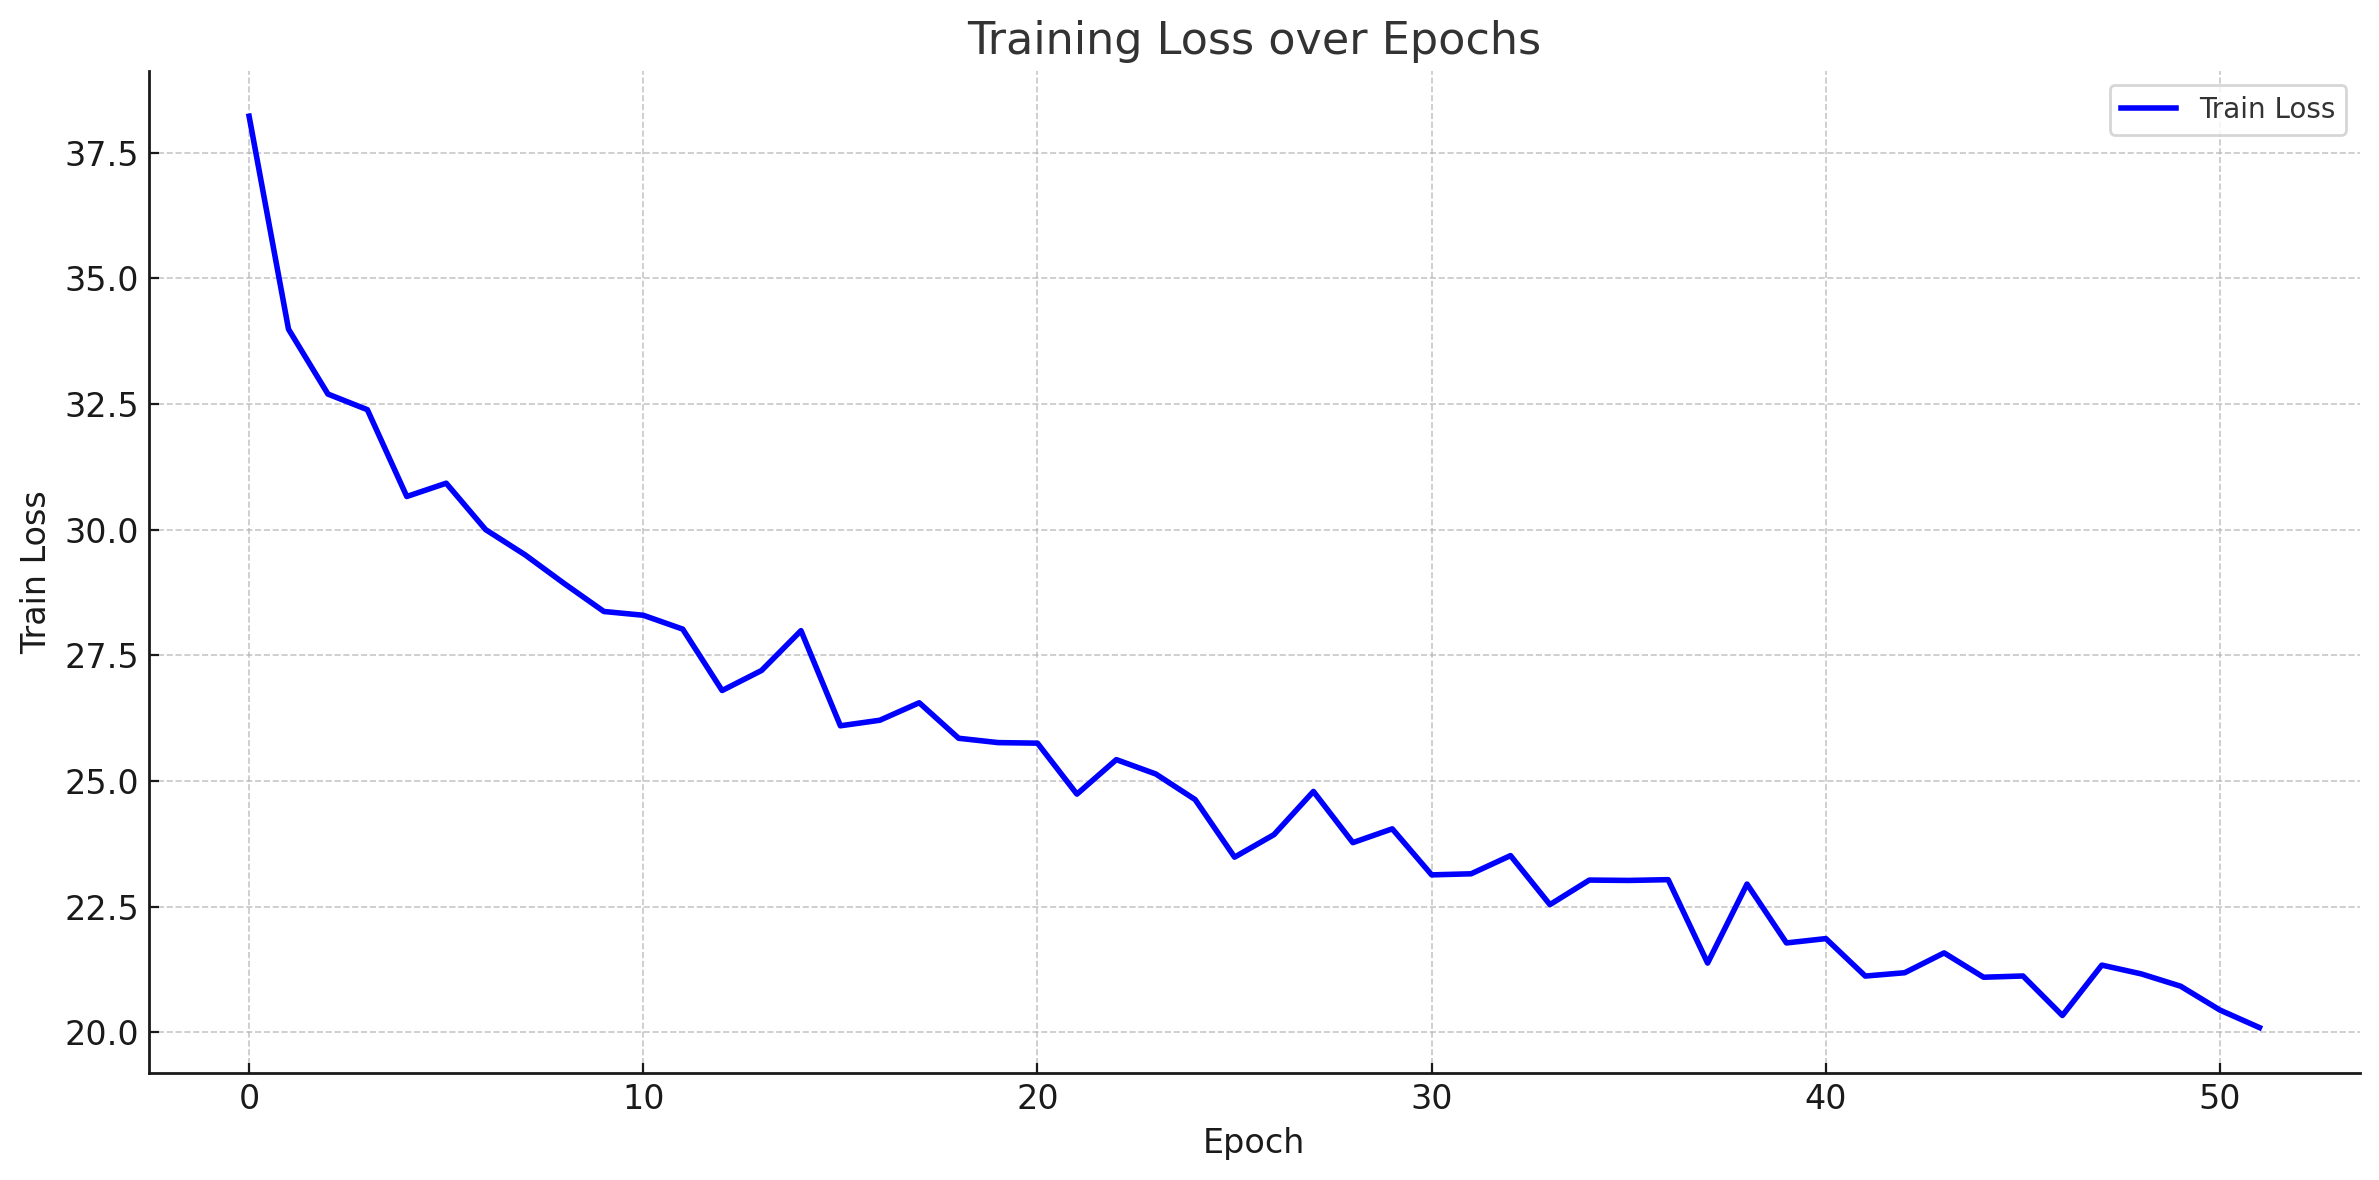
\includegraphics[width=\linewidth]{training_loss.png}
  \caption{Training loss and class accuracy over epochs. The plot shows a consistent decrease in loss and a gradual increase in accuracy, indicating effective learning.}
  \label{fig:training_loss}
\end{figure}

\subsection{YOLOv5s}
We achieved a mAP score of 34.1 with our YOLO5s model pre-trained on the COCO80 dataset and a training loss of 2.7. We were able to plot a confusion matrix for training and found that our model mistakenly confused a cross walk for a background object 56\% of the time and stairs as background objects 71\% of the time. However, it was accurately able to detect chimneys as true chimneys in the image 86\% of the time.
\begin{figure}[h!]
  \centering
  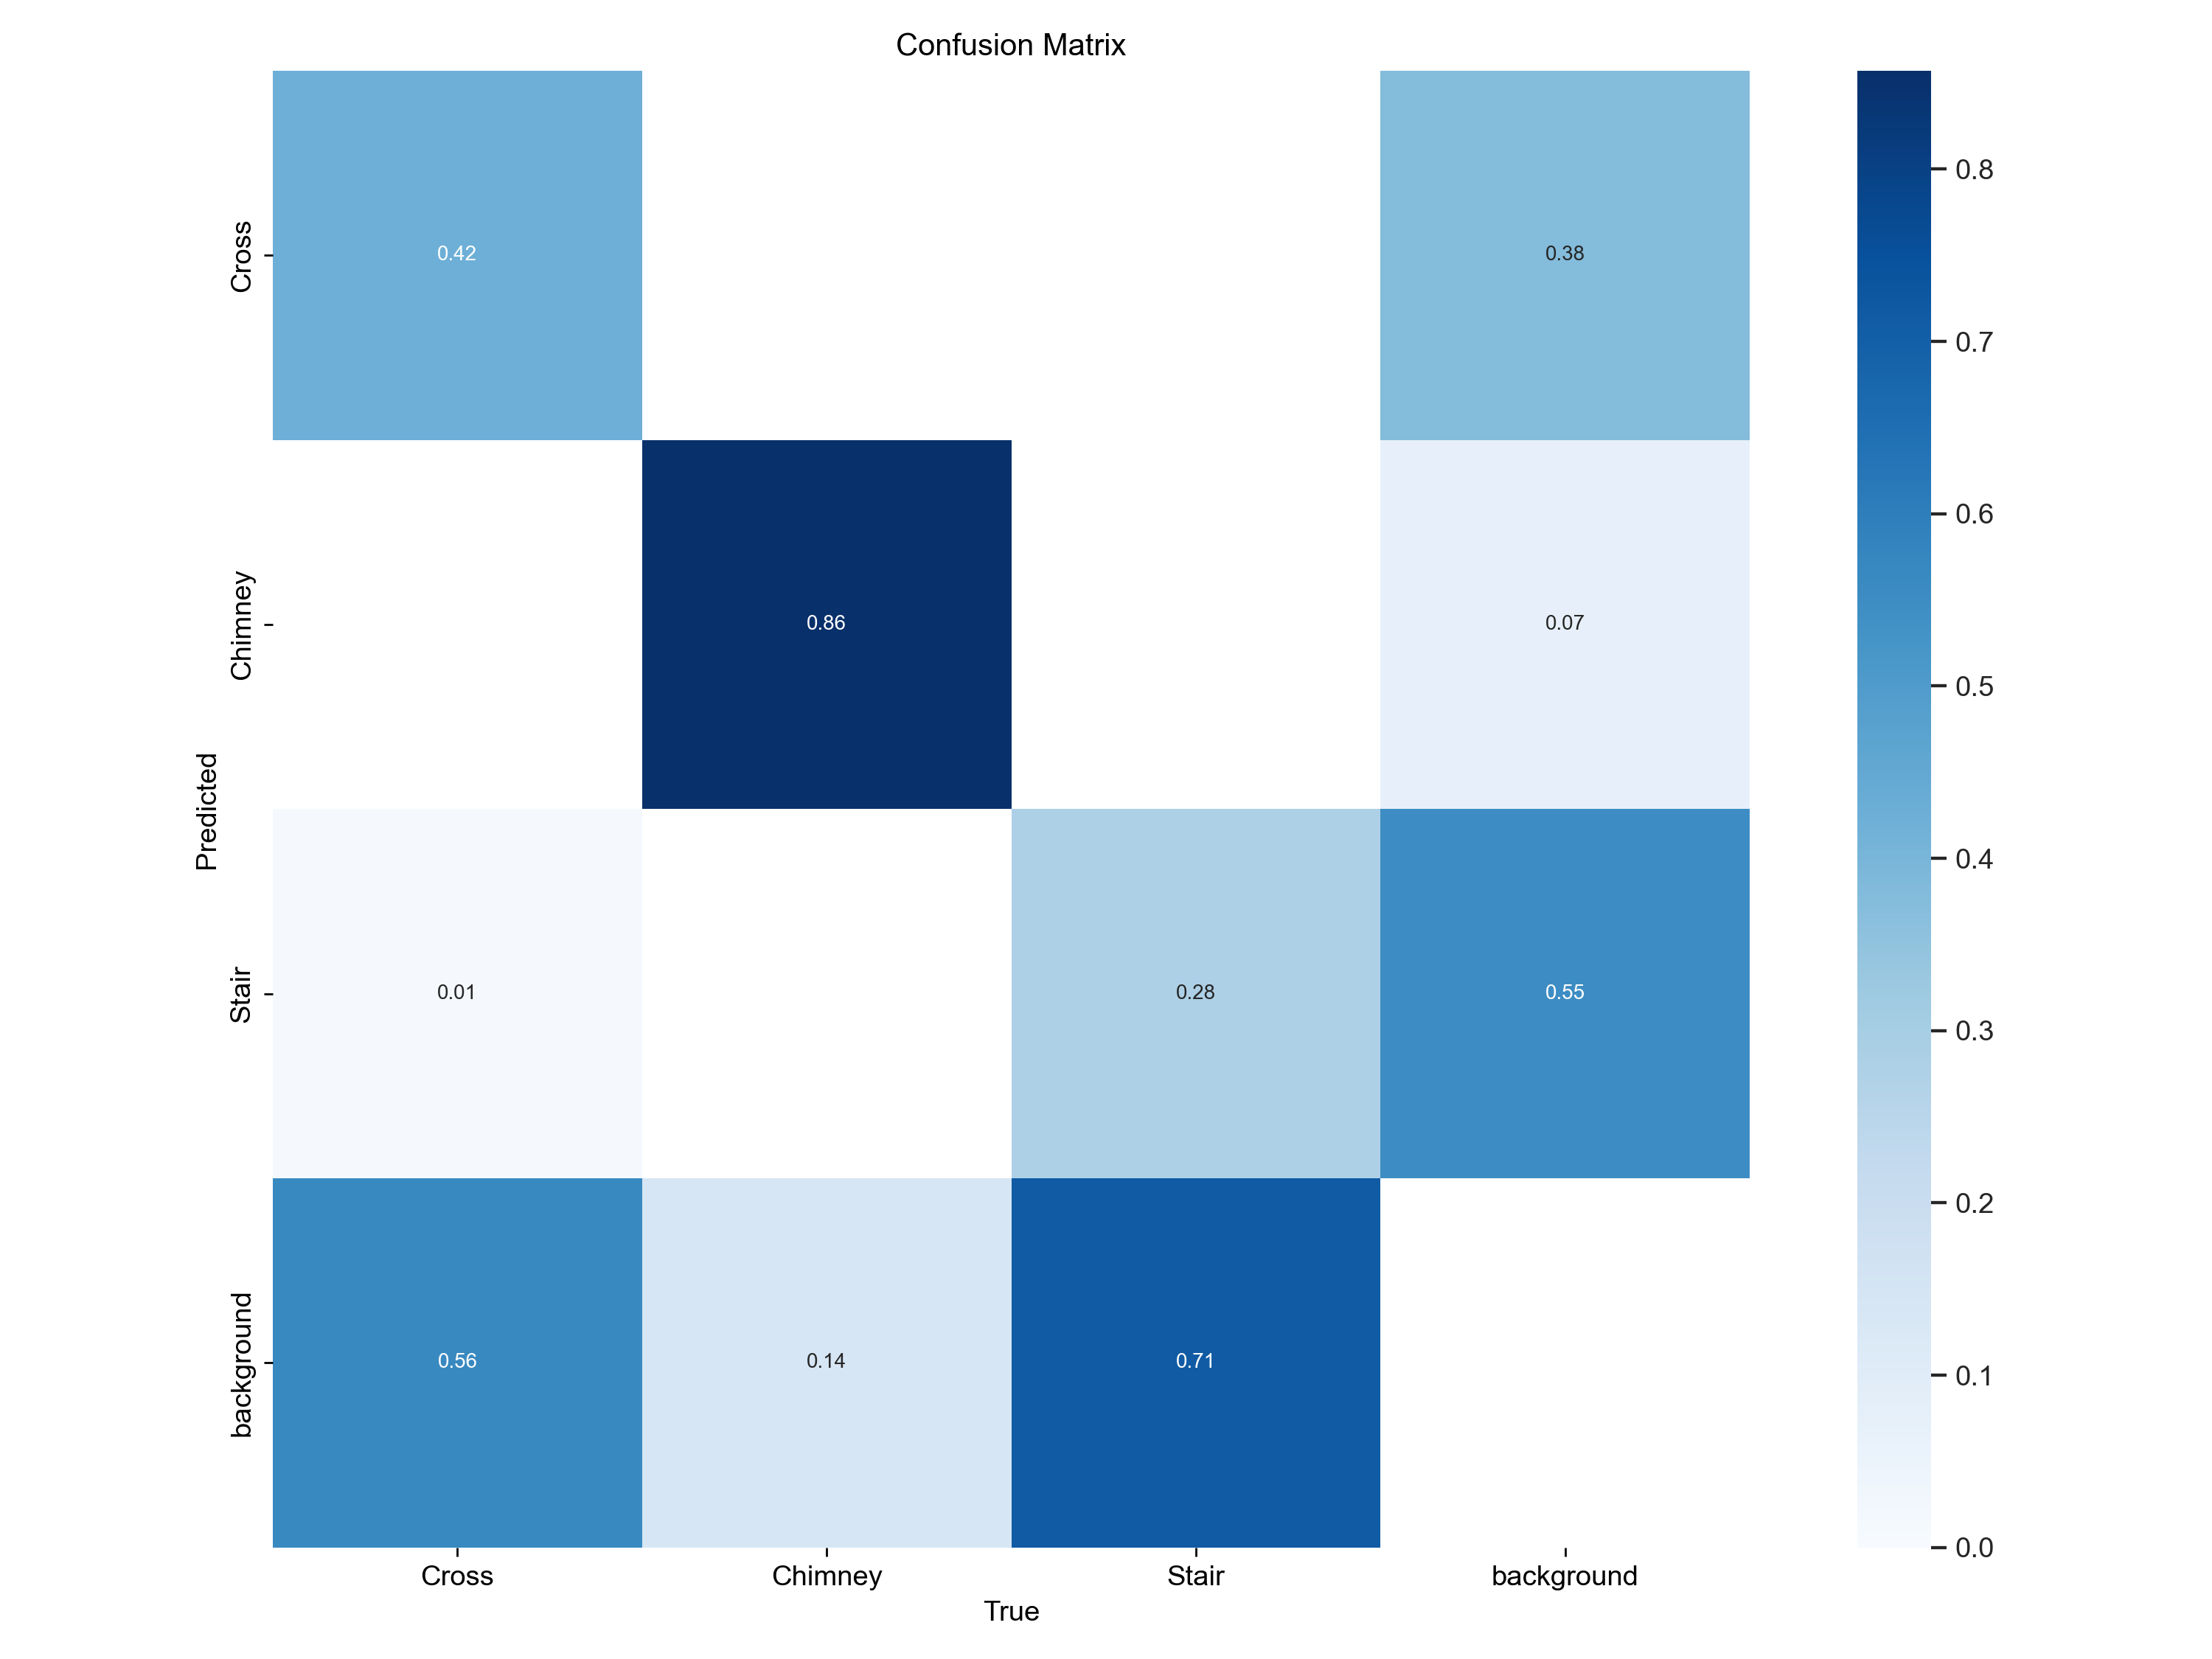
\includegraphics[width=\linewidth]{confusion_matrix.png}
  \caption{Confusion matrix showing model performance across classes. Darker diagonal elements indicate better classification accuracy for those classes.}
  \label{fig:confusion_matrix}
\end{figure}
\begin{figure}[h!]
  \centering
  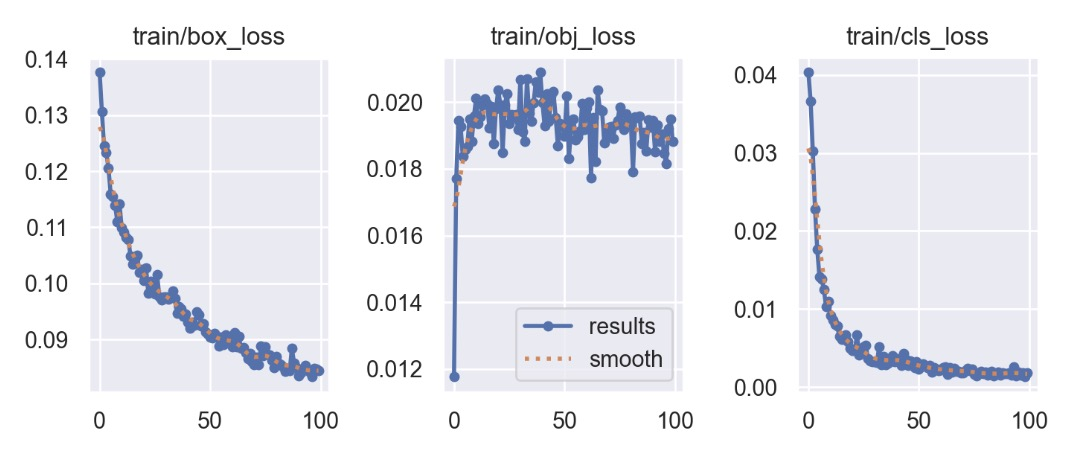
\includegraphics[width=\linewidth]{tl_loss.jpg}
  \caption{A collection of training losses including box coordinate accuracy loss, object accuracy loss, and class accuracy loss}
  \label{fig:training_losses}
\end{figure}

\section{Discussion}
\label{discussion}
Although our YOLOv5s model, trained using transfer learning, achieved a higher mAP score, it underperformed on a novel image set containing Chimneys and Stairs when compared to our custom YOLOv3 model evaluated on the same data. While the YOLOv5s model produced larger bounding boxes that more fully encompassed the target objects, our custom YOLOv3 demonstrated better precision in detecting Chimneys and Stairs. Conversely, YOLOv5s outperformed our model on Crosswalks, likely due to its pretrained weights from the full 200k annotated image set, in contrast to the limited subset used for training our custom model. The YOLOv5s model showed strong object recognition capabilities but exhibited signs of overfitting, generating more false positives than our model, which had been trained on only 500 annotated images spanning three specific classes from the COCO80 dataset. Our custom model, by comparison, likely underfitted the data due to the limited training set and narrower class coverage.

\begin{figure}[htbp]
  \centering
  \begin{subfigure}{\textwidth}
    \centering
    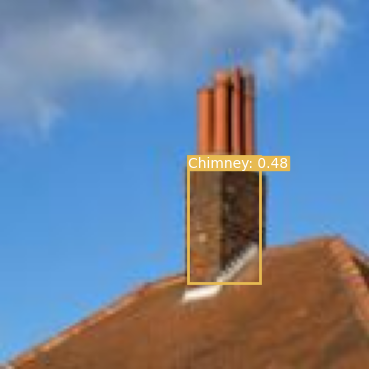
\includegraphics[width=0.7\linewidth]{Chimney (105)_nms.png}
    \caption{Custom YOLOv3 prediction on a Chimney (105)}
    \label{fig:chimney_nms}
  \end{subfigure}
  \hfill
  \begin{subfigure}{\textwidth}
    \centering
    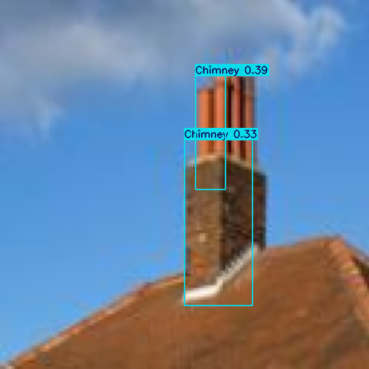
\includegraphics[width=0.7\linewidth]{Chimney (105)_tl.png}
    \caption{YOLOv5s Transfer Learning prediction on a Chimney (105)}
    \label{fig:chimney_tl}
  \end{subfigure}
  \label{fig:chimney_comparison}
\end{figure}

\begin{figure}[htbp]
  \centering
  \begin{subfigure}[\textwidth]
    \centering
    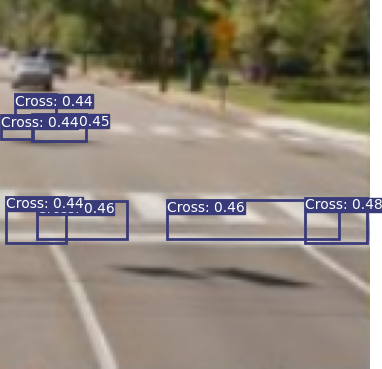
\includegraphics[width=\linewidth]{Cross (85)_nms.png}
    \caption{Custom YOLOv3 prediction on a Cross Walk (85)}
    \label{fig:cross_nms}
  \end{subfigure}
  \hfill
  \begin{subfigure}[\textwidth]
    \centering
    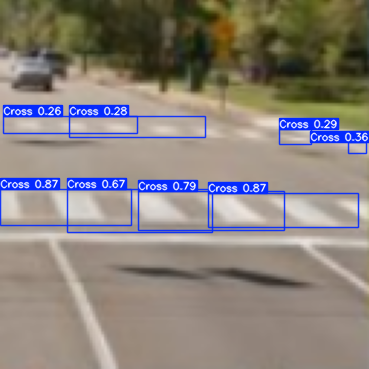
\includegraphics[width=\linewidth]{Cross (85)_tl.png}
    \caption{YOLOv5s Transfer Learning prediction on a Cross Walk (85)}
    \label{fig:cross_tl}
  \end{subfigure}
  \label{fig:cross_comparison}
\end{figure}

\subsection{Social Implications}
The social implications of our findings are largely positive, as these types of projects can contribute to societal benefits, such as improving navigation and reducing crime. However, there are systems that deploy this technology without the consent of those affected. Moreover, relying solely on this technology without human involvement is problematic, as AI models are not perfect and require significant oversight and quality data to function effectively.

\section{Conclusion}
\label{conclusion}

Despite the limitations of our small and imbalanced dataset, our fine-tuned YOLOv3 model demonstrated the ability to learn and distinguish between specific object classes, particularly chimneys, stairs, and crosswalks, within the Google reCAPTCHA V2 dataset. While the model achieved reasonable performance, our mAP score of 29.12 was lower compared to the performance obtained through transfer learning on the same dataset, indicating that there is room for further improvement.

\subsection{Future Work}

With more time, our future efforts will focus on more extensive hyperparameter tuning, particularly around confidence thresholds, Non-Maximum Suppression (NMS) thresholds, Intersection over Union (IoU) thresholds, and image resolutions. Additionally, we wish to expand the reCAPTCHA V2 dataset, both in size and class diversity, as the current dataset is limited to only three object types.

We also aim to explore real-world applications of our model, including developing a browser extension to automate reCAPTCHA v2 solving or adapting the model for video-based object detection tasks.

\section*{Acknowledgments}
We want to thank Professor Benjamin Mitchell for providing guidance at the start of our project.

% In the unusual situation where you want a paper to appear in the
% references without citing it in the main text, use \nocite
\nocite{langley00}

\bibliographystyle{icml2014}
\begin{thebibliography}{99}

\bibitem{felzenszwalb2008discriminatively}
Pedro~F. Felzenszwalb, Ross~B. Girshick, David McAllester, and Deva Ramanan.
\newblock Discriminatively trained deformable part models.
\newblock {\em IEEE Transactions on Pattern Analysis and Machine Intelligence}, 32(9):1627--1645, 2010.

\bibitem{girshick2014rich}
Ross Girshick, Jeff Donahue, Trevor Darrell, and Jitendra Malik.
\newblock Rich feature hierarchies for accurate object detection and semantic segmentation.
\newblock In {\em Proceedings of the IEEE Conference on Computer Vision and Pattern Recognition}, pages 580--587, 2014.

\bibitem{redmon2018yolov3}
Joseph Redmon and Ali Farhadi.
\newblock YOLOv3: An incremental improvement.
\newblock {\em arXiv preprint arXiv:1804.02767}, 2018.

\bibitem{ultralytics2020yolov5}
Ultralytics.
\newblock YOLOv5 in PyTorch.
\newblock \url{https://github.com/ultralytics/yolov5}, 2020.

\bibitem{persson2021darknet53}
Aladdin Persson.
\newblock YOLOv3 from scratch - Object Detection with PyTorch.
\newblock \url{https://www.youtube.com/watch?v=Grir6TZbc1M}, 2021.

\end{thebibliography}



\end{document}


% This document was modified from the file originally made available by
% Pat Langley and Andrea Danyluk for ICML-2K. This version was
% created by Lise Getoor and Tobias Scheffer, it was slightly modified
% from the 2010 version by Thorsten Joachims & Johannes Fuernkranz,
% slightly modified from the 2009 version by Kiri Wagstaff and
% Sam Roweis's 2008 version, which is slightly modified from
% Prasad Tadepalli's 2007 version which is a lightly
% changed version of the previous year's version by Andrew Moore,
% which was in turn edited from those of Kristian Kersting and
% Codrina Lauth. Alex Smola contributed to the algorithmic style files.